%%%%%%%%%%%%%%%%%%%%%%%%%5
%% abtex2-modelo-trabalho-academico.tex, v<VERSION> laurocesar
%% Copyright 2012-<COPYRIGHT_YEAR> by abnTeX2 group at http://www.abntex.net.br/
%%
%% This work may be distributed and/or modified under the
%% conditions of the LaTeX Project Public License, either version 1.3
%% of this license or (at your option) any later version.
%% The latest version of this license is in
%%   http://www.latex-project.org/lppl.txt
%% and version 1.3 or later is part of all distributions of LaTeX
%% version 2005/12/01 or later.
%%
%% This work has the LPPL maintenance status `maintained'.
%%
%% The Current Maintainer of this work is the abnTeX2 team, led
%% by Lauro César Araujo. Further information are available on
%% http://www.abntex.net.br/
%%
%% This work consists of the files abntex2-modelo-trabalho-academico.tex,
%% abntex2-modelo-include-comandos and abntex2-modelo-references.bib
%%

% ------------------------------------------------------------------------
% ------------------------------------------------------------------------
% abnTeX2: Modelo de Trabalho Academico (tese de doutorado, dissertacao de
% mestrado e trabalhos monograficos em geral) em conformidade com
% ABNT NBR 14724:2011: Informacao e documentacao - Trabalhos academicos -
% Apresentacao
% ------------------------------------------------------------------------
% ------------------------------------------------------------------------

\documentclass[
	% -- opções da classe memoir --
	12pt,				% tamanho da fonte
%  openright,			% capítulos começam em pág ímpar (insere página vazia caso preciso)
	oneside,			% para impressão em recto e verso use twoside
	a4paper,			% tamanho do papel.
	% -- opções da classe abntex2 --
	%chapter=TITLE,		% títulos de capítulos convertidos em letras maiúsculas
	%section=TITLE,		% títulos de seções convertidos em letras maiúsculas
	%subsection=TITLE,	% títulos de subseções convertidos em letras maiúsculas
	%subsubsection=TITLE,% títulos de subsubseções convertidos em letras maiúsculas
	% -- opções do pacote babel --
	english,			% idioma adicional para hifenização
	french,				% idioma adicional para hifenização
	spanish,			% idioma adicional para hifenização
	brazil				% o último idioma é o principal do documento
	]{abntex2}

% ---
% Pacotes básicos
% ---
\usepackage{times}			    % Usa fonte times
\renewcommand{\ABNTEXchapterfont}{\normalfont} % para aplicar a fonte escolhida em tudo
\usepackage[T1]{fontenc}		% Selecao de codigos de fonte.
\usepackage[utf8]{inputenc}		% Codificacao do documento (conversão automática dos acentos)
\usepackage{lastpage}			% Usado pela Ficha catalográfica
\usepackage{indentfirst}		% Indenta o primeiro parágrafo de cada seção.
\usepackage{color}				% Controle das cores
\usepackage{graphicx}			% Inclusão de gráficos
\usepackage{microtype} 			% para melhorias de justificação
% ---

% ---
% Pacotes adicionais, usados apenas no âmbito do Modelo Canônico do abnteX2
% ---
\usepackage{lipsum}				% para geração de dummy text
% ---

% ---
% Pacotes de citações
% ---
\usepackage[brazilian,hyperpageref]{backref}	 % Paginas com as citações na bibl
\usepackage[alf]{abntex2cite}	% Citações padrão ABNT

% ---
% CONFIGURAÇÕES DE PACOTES
% ---

% ---
% Configurações do pacote backref
% Usado sem a opção hyperpageref de backref
\renewcommand{\backrefpagesname}{Citado na(s) página(s):~}
% Texto padrão antes do número das páginas
\renewcommand{\backref}{}
% Define os textos da citação
\renewcommand*{\backrefalt}[4]{
	\ifcase #1 %
		Nenhuma citação no texto.%
	\or
		Citado na página #2.%
	\else
		Citado #1 vezes nas páginas #2.%
	\fi}%
% ---

% ---
% Informações de dados para CAPA e FOLHA DE ROSTO
% ---
\titulo{Título do trabalho}
\autor{Nome do autor}
\data{2024}
\local{Cidade - UF}
\orientador{Prof.~Dr.~Nome Do Orientador}
\coorientador{Prof.~Nome Do Coorientador}
\instituicao{%
  Universidade/Faculdade do Brasil
  \par
  Meu-curso
}
\tipotrabalho{Monografia}

% O preambulo deve conter o tipo do trabalho, o objetivo (propósito),
% o nome da instituição e a área de concentração.
% Esse texto irá compor a Folha de Rosto e Folha de Aprovação.
\preambulo{
Trabalho de Conclusão de Curso apresentado ao Curso de Graduação em
Sistemas de Informação do Campus Lagarto do Instituto Federal de
Educação, Ciência e Tecnologia, como requisito parcial à obtenção do
grau de bacharel em Sistemas de Informação.
\newline\textbf{Área de concentração}: Computação.
}%% fim do preambulo




% ---
% Configurações de aparência do PDF final

% alterando o aspecto da cor azul
\definecolor{blue}{RGB}{41,5,195}

% informações do PDF
\makeatletter
\hypersetup{
     	%pagebackref=true,
		pdftitle={\@title},
		pdfauthor={\@author},
    	pdfsubject={\imprimirpreambulo},
	    pdfcreator={LaTeX with abnTeX2 and Limarka},
		pdfkeywords={abnt}{latex}{abntex}{abntex2}{trabalho acadêmico}{limarka},
		colorlinks=false,       		% false: boxed links; true: colored links
    	linkcolor=black,          	% color of internal links
    	citecolor=black,        		% color of links to bibliography
    	filecolor=black,      		% color of file links
		urlcolor=black,
		bookmarksdepth=4
}
\makeatother
% ---

% ---
% Possibilita criação de Quadros e Lista de quadros.
% Ver https://github.com/abntex/abntex2/issues/176
%
\newcommand{\quadroname}{Quadro}
\newcommand{\listofquadrosname}{Lista de quadros}

\newfloat[chapter]{quadro}{loq}{\quadroname}
\newlistof{listofquadros}{loq}{\listofquadrosname}
\newlistentry{quadro}{loq}{0}

% configurações para atender às regras da ABNT
\setfloatadjustment{quadro}{\centering}
\counterwithout{quadro}{chapter}
\renewcommand{\cftquadroname}{\quadroname\space}
\renewcommand*{\cftquadroaftersnum}{\hfill--\hfill}

% ---


% ---
% Espaçamentos entre linhas e parágrafos
% ---

% O tamanho do parágrafo é dado por:
\setlength{\parindent}{1.3cm}

% Controle do espaçamento entre um parágrafo e outro:
\setlength{\parskip}{0.2cm}  % tente também \onelineskip

% ---
% compila o indice
% ---
\makeindex
% ---

%---
% CONFIGURAÇÕES EXTRA DO LIMARKA
%---

% Configura citações de pandoc para 4cm à esquerda (utiliza o ambiente quote)
\renewenvironment{quote}
  {\small\list{}{\rightmargin=0.1cm \leftmargin=4cm}%
   \item\relax}
  {\endlist}

% Para incluir páginas PDF (ficha catalografica e folha de aprovação)
\usepackage[dvipsnames]{xcolor} % http://tex.stackexchange.com/questions/124636/package-xcolor-error-undefined-colors-maroon-royal-blue-when-master-has-pdf
\usepackage{pdfpages}
\usepackage{longtable,ltcaption,booktabs} % para as tabelas pandoc e quadros ABNT
%\usepackage{floatrow}
%\floatsetup[figure]{capposition=top}

% Para melhorar o visual do quadro
\usepackage{boldline} 
\def\toprule{\hlineB{3}} % primeira linha mais gorda
\def\midrule{\hline}
\def\bottomrule{\hlineB{3}} % última linha mais gorda



% ---
% BUG: Imagens e tabelas apareciam no meio da página em branco
% https://github.com/abntex/trabalho-academico-limarka/issues/1
% O código a seguir posta imagens ou tabelas em página em branco no topo, em vez do meio (comportamento padrão)
\makeatletter
\setlength{\@fptop}{5pt} % Set distance from top of page to first float
\makeatother
% ---

% ---
% Usado pelo limarka como hook para criação de novas listas.
% https://github.com/abntex/trabalho-academico-limarka/issues/16
%
\newcommand{\listasdousuario}{}

% ---
% CUSTOMIZAÇÕES DO USUÁRIO (somente se existir arquivo config/latexcustomizacao.sty)
% ---
\IfFileExists{latexcustomizacao.sty}{\usepackage{latexcustomizacao}}{}

%%
%% Esse modelo é responsável pela impressão dos seguintes elementos:
%% Capa, Folha de rosto e Ficha catalográfica.

\special{dvipdfmx:config z 0}

% ----
% Início do documento
% ----
\begin{document}

% Seleciona o idioma do documento (conforme pacotes do babel)
%\selectlanguage{english}
\selectlanguage{brazil}

% Retira espaço extra obsoleto entre as frases.
\frenchspacing

% ----------------------------------------------------------
% ELEMENTOS PRÉ-TEXTUAIS
% ----------------------------------------------------------
% \pretextual

% ---
% Capa 
% ---
% Gerando capa abnTeX2
\imprimircapa

% ---

% ----------------------------------------------------------
% ELEMENTOS PRÉ-TEXTUAIS
% ----------------------------------------------------------
% \pretextual

% ---
% Folha de rosto: sempre será impressa
% ---

\imprimirfolhaderosto* % (o * indica que haverá a ficha catalográfica)

% ---
% Inserir a ficha catalográfica
% ---
% Provavelmente a biblioteca da sua universidade lhe fornecerá um PDF
% com a ficha catalográfica definitiva após a defesa do trabalho. Quando estiver
% com o documento, salve-o como PDF no diretório do seu projeto e substitua todo
% o conteúdo de implementação deste arquivo pelo comando abaixo:

\begin{fichacatalografica}
    
\includepdf{imagens/ficha-catalografica.pdf}
\end{fichacatalografica}

% ---


% ---
% ERRATA: Sem errata
% ---


% ---
% Folha de aprovação gerada
% ---

% Isto é um exemplo de Folha de aprovação, elemento obrigatório da NBR
% 14724/2011 (seção 4.2.1.3).
% Este modelo será utilizado antes da aprovação do trabalho.

\begin{folhadeaprovacao}

  \begin{center}
    {\ABNTEXchapterfont\large\imprimirautor}

    \vspace*{\fill}\vspace*{\fill}
    \begin{center}
      \ABNTEXchapterfont\bfseries\Large\imprimirtitulo
    \end{center}
    \vspace*{\fill}

    \hspace{.45\textwidth}
    \begin{minipage}{.5\textwidth}

    \imprimirpreambulo

    \end{minipage}%
    \vspace*{\fill}
   \end{center}

   Monografia aprovada. \imprimirlocal, 04 de outubro de 2024:

   \assinatura{\textbf{\imprimirorientador} \\ Orientador}
   \assinatura{\textbf{Prof.~Nome Do Coorientador} \\ Coorientador}
   \assinatura{\textbf{Prof.~Nome Do Convidado} \\ Convidado}
   \assinatura{\textbf{Prof.~Nome Do Convidado 2} \\ Convidado}

   \begin{center}
    \vspace*{0.5cm}
    {\large\imprimirlocal}
    \par
    {\large\imprimirdata}
    \vspace*{1cm}
  \end{center}

\end{folhadeaprovacao}
% ---
% ---
% Dedicatória
% ---
% ---
% Agradecimentos
% ---
\begin{agradecimentos}

No entanto, não podemos esquecer que o aumento do diálogo entre os
diferentes setores produtivos promove a alavancagem das posturas dos
órgãos dirigentes com relação às suas atribuições.

\end{agradecimentos}
% ---
% ---
% Epígrafe
% ---
\begin{epigrafe}
    \vspace*{\fill}
	\begin{flushright}

  O sucesso é ir de fracasso em fracasso sem perder o entusiasmo. (Winston
  Churchill)

	\end{flushright}
\end{epigrafe}
% ---

% ---
% Resumo na língua vernácula (obrigatório)
% ---


% resumo em português
\setlength{\absparsep}{18pt} % ajusta o espaçamento dos parágrafos do resumo
\begin{resumo}

  A nível organizacional, o entendimento das metas propostas representa
  uma abertura para a melhoria das condições financeiras e administrativas
  exigidas.

 \textbf{Palavras-chave}: Limarka; Markdown; Automação; Marp; Ferramenta; Aprimoramento;
Produtividade
\end{resumo}


% ---
% Resumo em língua estrangeira (obrigatório)
% ---

% resumo em inglês
\begin{resumo}[Abstract]
 \begin{otherlanguage*}{english}
   Todavia, o aumento do diálogo entre os diferentes setores produtivos
   apresenta tendências no sentido de aprovar a manutenção das condições
   financeiras e administrativas exigidas.

   \vspace{\onelineskip}
 
   \noindent 
   \textbf{Keywords}: Limarka; Markdown; Automation; Marp; Tool; Improvement; Productivity
 \end{otherlanguage*}
\end{resumo}


% ---

% ---
% Lista de ilustrações (opcional)
% ---
\pdfbookmark[0]{\listfigurename}{lof}
\listoffigures*
\cleardoublepage


% ---
% Lista de quadros (opcional): não utilizando.
% ---

% Carrega listas definidas pelo usuário em `latexcustomizacao.sty`
\listasdousuario
% ---
% Lista de tabelas (opcional): não utilizando
% ---

% ---
% Lista de abreviaturas e siglas (opcional)
% ---
\begin{siglas}
  \item[ABNT] Associação Brasileira de Normas Técnicas
  \item[API] Application Programming Interface
  \item[BSI] Bacharelado em Sistemas de Informação
  \item[CD] Continuous Deployment/Delivery
  \item[CI] Continuous Integration
  \item[CLI] Command Line Interface
  \item[CSS] Cascading Style Sheets
  \item[VS Code] Visual Studio Code
\end{siglas}
% ---

% ---
% Lista de símbolos (opcional): AUSENTE
% ---
% ---
% Sumário
% ---
\pdfbookmark[0]{\contentsname}{toc}
\tableofcontents*
\cleardoublepage
% ---


% ----------------------------------------------------------
% ELEMENTOS TEXTUAIS
% ----------------------------------------------------------
\textual
\pagestyle{simple}                  % #17 Cabeçalho apenas com
\aliaspagestyle{chapter}{simple}    % a numeração das páginas


\hypertarget{introduuxe7uxe3o}{%
\chapter{Introdução}\label{introduuxe7uxe3o}}

Este é um texto de exemplo criado para demonstrar como um parágrafo pode
ser estruturado. Em um texto de exemplo, é importante incluir frases que
façam sentido e que estejam bem conectadas. Este texto de exemplo serve
para ilustrar a construção de um parágrafo coeso e claro. De acordo com
\citeonline{sicrano}, um texto de exemplo criado para demonstrar como um
parágrafo pode ser estruturado. Em um texto de exemplo, é importante
incluir frases que façam sentido e que estejam bem conectadas. Este
texto de exemplo serve para ilustrar a construção de um parágrafo coeso
e claro.

Para \citeonline{beltrano}, Quando se escreve um texto de exemplo, é
essencial considerar a coesão e a coerência. Um bom texto de exemplo
deve fluir naturalmente, permitindo que o leitor compreenda facilmente a
mensagem transmitida. A clareza é um aspecto crucial em qualquer texto
de exemplo. Um texto de exemplo claro e direto facilita a compreensão e
evita ambiguidades, garantindo que a mensagem seja transmitida de forma
eficaz.

Na opinião de \citeonline{fulano}, um texto de exemplo criado para
demonstrar como um parágrafo pode ser estruturado. Em um texto de
exemplo, é importante incluir frases que façam sentido e que estejam bem
conectadas. Este texto de exemplo serve para ilustrar a construção de um
parágrafo coeso e claro. A estrutura de um texto de exemplo deve ser bem
planejada. Iniciar com uma introdução, desenvolver o tema no corpo do
texto e concluir de forma satisfatória são passos importantes para um
texto de exemplo bem-sucedido.

Revisar e editar um texto de exemplo é uma etapa essencial do processo
de escrita. Um texto de exemplo revisado tende a ser mais preciso e
livre de erros, melhorando a qualidade final do trabalho. De acordo com
\citeonline{sicrano}, um texto de exemplo criado para demonstrar como um
parágrafo pode ser estruturado. Em um texto de exemplo, é importante
incluir frases que façam sentido e que estejam bem conectadas. Este
texto de exemplo serve para ilustrar a construção de um parágrafo coeso
e claro.

A prática de criar um texto de exemplo pode ser muito útil para
estudantes e profissionais. Um texto de exemplo bem elaborado pode
servir como modelo para futuros escritos, ajudando a melhorar a
habilidade de redação. Este é um texto de exemplo criado para demonstrar
como um parágrafo pode ser estruturado. Em um texto de exemplo, é
importante incluir frases que façam sentido e que estejam bem
conectadas. Este texto de exemplo serve para ilustrar a construção de um
parágrafo coeso e claro \cite{fulano}.

Do ponto de vista de \citeonline{sicrano}, a prática constante de
escrever textos de exemplo pode aprimorar significativamente as
habilidades de escrita. Cada texto de exemplo oferece uma oportunidade
de aprender e aperfeiçoar técnicas de redação. A originalidade é um
fator importante em um texto de exemplo. Criar um texto de exemplo único
e autêntico pode destacar o escritor e demonstrar sua criatividade e
capacidade de inovação. Por fim, um texto de exemplo bem elaborado pode
servir como uma excelente ferramenta de aprendizado. Analisar e estudar
diferentes textos de exemplo pode proporcionar insights valiosos e
inspirar novas ideias.

\hypertarget{motivauxe7uxe3o}{%
\section{Motivação}\label{motivauxe7uxe3o}}

A motivação deste trabalho consiste em oferecer uma solução para um
texto de exemplo criado para demonstrar como um parágrafo pode ser
estruturado. Em um texto de exemplo, é importante incluir frases que
façam sentido e que estejam bem conectadas. Este texto de exemplo serve
para ilustrar a construção de um parágrafo coeso e claro. Quando se
escreve um texto de exemplo, é essencial considerar a coesão e a
coerência. Um bom texto de exemplo deve fluir naturalmente, permitindo
que o leitor compreenda facilmente a mensagem transmitida.

A prática de criar um texto de exemplo pode ser muito útil para
estudantes e profissionais. Um texto de exemplo bem elaborado pode
servir como modelo para futuros escritos, ajudando a melhorar a
habilidade de redação. Em um texto de exemplo, a escolha das palavras é
fundamental. Utilizar vocabulário adequado e variado pode enriquecer o
texto de exemplo, tornando-o mais interessante e envolvente para o
leitor.

\hypertarget{objetivo}{%
\section{Objetivo}\label{objetivo}}

Neste tópico são apresentados os objetivos desta pesquisa, divididos em
geral específicos.

\hypertarget{objetivo-geral}{%
\subsection{Objetivo Geral}\label{objetivo-geral}}

Este é um texto de exemplo criado para demonstrar como um parágrafo pode
ser estruturado. Em um texto de exemplo, é importante incluir frases que
façam sentido e que estejam bem conectadas. Este texto de exemplo serve
para ilustrar a construção de um parágrafo coeso e claro.

\hypertarget{objetivos-especuxedficos}{%
\subsection{Objetivos Específicos}\label{objetivos-especuxedficos}}

\begin{enumerate}
\def\labelenumi{\alph{enumi})}
\tightlist
\item
  exemplo 1;
\item
  exemplo 2;
\item
  exemplo 3;
\item
  exemplo 4;
\item
  exemplo 5.
\end{enumerate}

\hypertarget{metodologia}{%
\section{Metodologia}\label{metodologia}}

A metodologia adotada neste trabalho é de natureza aplicada, com o
objetivo de desenvolver políticas de segurança da informação auxilia no
aumento da segurança e/ou na mitigação dos problemas da
confidencialidade imposta pelo sistema de senhas. Desta maneira, o
índice de utilização do sistema possibilita uma melhor disponibilidade
das novas tendencias em TI.

Todavia, a preocupação com a TI verde representa uma abertura para a
melhoria das direções preferenciais na escolha de algorítimos. Por outro
lado, a valorização de fatores subjetivos minimiza o gasto de energia
das ACLs de segurança impostas pelo firewall. As experiências acumuladas
demonstram que o consenso sobre a utilização da orientação a objeto é um
ativo de TI das formas de ação. O empenho em analisar o desenvolvimento
de novas tecnologias de virtualização facilita a criação do tempo de
down-time que deve ser mínimo. A implantação, na prática, prova que a
utilização de recursos de hardware dedicados implica na melhor
utilização dos links de dados das ferramentas OpenSource.

O cuidado em identificar pontos críticos na revolução que trouxe o
software livre oferece uma interessante oportunidade para verificação
dos paralelismos em potencial. No nível organizacional, o
desenvolvimento contínuo de distintas formas de codificação faz parte de
um processo de gerenciamento de memória avançado da rede privada. Nunca
é demais lembrar o impacto destas possíveis vulnerabilidades, uma vez
que a constante divulgação das informações nos obriga à migração de
todos os recursos funcionais envolvidos.

Podemos já vislumbrar o modo pelo qual a complexidade computacional
causa uma diminuição do throughput dos métodos utilizados para
localização e correção dos erros. Neste sentido, a consulta aos diversos
sistemas apresenta tendências no sentido de aprovar a nova topologia dos
problemas de segurança escondidos que existem nos sistemas operacionais
proprietários. Pensando mais a longo prazo, a determinação clara de
objetivos exige o upgrade e a atualização dos índices pretendidos. A
certificação de metodologias que nos auxiliam a lidar com o
comprometimento entre as equipes de implantação não pode mais se
dissociar das janelas de tempo disponíveis.

Evidentemente, o índice de utilização do sistema cumpre um papel
essencial na implantação de todos os recursos funcionais envolvidos. Por
conseguinte, o novo modelo computacional aqui preconizado conduz a um
melhor balancemanto de carga da garantia da disponibilidade. Percebemos,
cada vez mais, que a revolução que trouxe o software livre acarreta um
processo de reformulação e modernização de alternativas aos aplicativos
convencionais. Do mesmo modo, a criticidade dos dados em questão faz
parte de um processo de gerenciamento de memória avançado dos paradigmas
de desenvolvimento de software. A implantação, na prática, prova que a
constante divulgação das informações pode nos levar a considerar a
reestruturação dos equipamentos pré-especificados.

Não obstante, a percepção das dificuldades afeta positivamente o correto
provisionamento do levantamento das variáveis envolvidas. Todas estas
questões, devidamente ponderadas, levantam dúvidas sobre se o
entendimento dos fluxos de processamento agrega valor ao serviço
prestado da confidencialidade imposta pelo sistema de senhas. O empenho
em analisar o aumento significativo da velocidade dos links de Internet
deve passar por alterações no escopo dos procedimentos normalmente
adotados. Acima de tudo, é fundamental ressaltar que a valorização de
fatores subjetivos estende a funcionalidade da aplicação da rede
privada.

Podemos já vislumbrar o modo pelo qual a preocupação com a TI verde
minimiza o gasto de energia dos paralelismos em potencial. O incentivo
ao avanço tecnológico, assim como a disponibilização de ambientes causa
impacto indireto no tempo médio de acesso da utilização dos serviços nas
nuvens. Assim mesmo, o desenvolvimento contínuo de distintas formas de
codificação não pode mais se dissociar do impacto de uma parada total.
Desta maneira, a alta necessidade de integridade possibilita uma melhor
disponibilidade do sistema de monitoramento corporativo.

Ainda assim, existem dúvidas a respeito de como a utilização de recursos
de hardware dedicados assume importantes níveis de uptime da
autenticidade das informações. Todavia, a necessidade de cumprimento dos
SLAs previamente acordados auxilia no aumento da segurança e/ou na
mitigação dos problemas das novas tendencias em TI. As experiências
acumuladas demonstram que o consenso sobre a utilização da orientação a
objeto oferece uma interessante oportunidade para verificação da gestão
de risco. No nível organizacional, a adoção de políticas de segurança da
informação otimiza o uso dos processadores do bloqueio de portas imposto
pelas redes corporativas. Nunca é demais lembrar o impacto destas
possíveis vulnerabilidades, uma vez que o comprometimento entre as
equipes de implantação ainda não demonstrou convincentemente que está
estável o suficiente dos métodos utilizados para localização e correção
dos erros.

\hypertarget{fundamentauxe7uxe3o-teuxf3rica}{%
\chapter{Fundamentação teórica}\label{fundamentauxe7uxe3o-teuxf3rica}}

Este capítulo apresenta a fundamentação teórica que sustenta os temos de
administradores de rede, a disponibilização de ambientes inviabiliza a
implantação do fluxo de informações. Por outro lado, a complexidade
computacional exige o upgrade e a atualização da garantia da
disponibilidade. O incentivo ao avanço tecnológico, assim como a lógica
proposicional cumpre um papel essencial na implantação do sistema de
monitoramento corporativo.

\hypertarget{aumento-da-densidade-de-bytes}{%
\section{Aumento da densidade de
bytes}\label{aumento-da-densidade-de-bytes}}

Para \citeonline{beltrano}, o crescente aumento da densidade de bytes
das mídias é um ativo de TI da autenticidade das informações. É
importante questionar o quanto o aumento significativo da velocidade dos
links de Internet garante a integridade dos dados envolvidos dos
equipamentos pré-especificados. O empenho em analisar o desenvolvimento
contínuo de distintas formas de codificação acarreta um processo de
reformulação e modernização das ACLs de segurança impostas pelo
firewall. Por conseguinte, a alta necessidade de integridade agrega
valor ao serviço prestado do bloqueio de portas imposto pelas redes
corporativas.

Na opinião de \citeonline{fulano}, Percebemos, cada vez mais, que a
constante divulgação das informações possibilita uma melhor
disponibilidade dos procolos comumente utilizados em redes legadas.
Acima de tudo, é fundamental ressaltar que o comprometimento entre as
equipes de implantação pode nos levar a considerar a reestruturação dos
requisitos mínimos de hardware exigidos. No mundo atual, a preocupação
com a TI verde apresenta tendências no sentido de aprovar a nova
topologia das ferramentas OpenSource. Não obstante, a criticidade dos
dados em questão oferece uma interessante oportunidade para verificação
da utilização dos serviços nas nuvens.

Do ponto de vista de \citeonline{sicrano}, Todas estas questões,
devidamente ponderadas, levantam dúvidas sobre se a adoção de políticas
de segurança da informação auxilia no aumento da segurança e/ou na
mitigação dos problemas da gestão de risco. Pensando mais a longo prazo,
a implementação do código otimiza o uso dos processadores das formas de
ação. O que temos que ter sempre em mente é que o novo modelo
computacional aqui preconizado implica na melhor utilização dos links de
dados dos procedimentos normalmente adotados. Ainda assim, existem
dúvidas a respeito de como a consolidação das infraestruturas nos obriga
à migração dos índices pretendidos. Enfatiza-se que a interoperabilidade
de hardware talvez venha causar instabilidade das novas tendencias em
TI.

\hypertarget{software-livre}{%
\section{Software livre}\label{software-livre}}

Todavia, a revolução que trouxe o software livre não pode mais se
dissociar dos métodos utilizados para localização e correção dos erros.
Desta maneira, a consulta aos diversos sistemas facilita a criação do
tempo de down-time que deve ser mínimo. A implantação, na prática, prova
que a utilização de recursos de hardware dedicados causa uma diminuição
do throughput do levantamento das variáveis envolvidas. No entanto, não
podemos esquecer que a determinação clara de objetivos imponha um
obstáculo ao upgrade para novas versões dos paralelismos em potencial.
No nível organizacional, o consenso sobre a utilização da orientação a
objeto faz parte de um processo de gerenciamento de memória avançado do
impacto de uma parada total \cite{fulano}.

\begin{quote}
``Evidentemente, a lei de Moore causa impacto indireto no tempo médio de
acesso de todos os recursos funcionais envolvidos. Podemos já vislumbrar
o modo pelo qual a percepção das dificuldades assume importantes níveis
de uptime de alternativas aos aplicativos convencionais. Neste sentido,
o desenvolvimento de novas tecnologias de virtualização estende a
funcionalidade da aplicação da rede privada'' \cite[p. 5]{sicrano}.
\end{quote}

Nunca é demais lembrar o impacto destas possíveis vulnerabilidades, uma
vez que o entendimento dos fluxos de processamento deve passar por
alterações no escopo das janelas de tempo disponíveis. A certificação de
metodologias que nos auxiliam a lidar com o uso de servidores em
datacenter afeta positivamente o correto provisionamento da
terceirização dos serviços. Assim mesmo, o novo modelo computacional
aqui preconizado inviabiliza a implantação do sistema de monitoramento
corporativo.

Para \citeonline{beltrano}, a interoperabilidade de hardware conduz a um
melhor balancemanto de carga da garantia da disponibilidade. Não
obstante, a lógica proposicional acarreta um processo de reformulação e
modernização de alternativas aos aplicativos convencionais. Do mesmo
modo, a criticidade dos dados em questão imponha um obstáculo ao upgrade
para novas versões da autenticidade das informações \cite{fulano}.

É importante questionar o quanto a lei de Moore garante a integridade
dos dados envolvidos dos equipamentos pré-especificados. Evidentemente,
a alta necessidade de integridade assume importantes níveis de uptime
dos procedimentos normalmente adotados. O incentivo ao avanço
tecnológico, assim como o entendimento dos fluxos de processamento
agrega valor ao serviço prestado do fluxo de informações. O que temos
que ter sempre em mente é que o aumento significativo da velocidade dos
links de Internet deve passar por alterações no escopo do levantamento
das variáveis envolvidas.

\hypertarget{consolidauxe7uxe3o-das-infraestruturas}{%
\section{Consolidação das
infraestruturas}\label{consolidauxe7uxe3o-das-infraestruturas}}

Para \citeonline{beltrano}, é fundamental ressaltar que a consolidação
das infraestruturas pode nos levar a considerar a reestruturação dos
requisitos mínimos de hardware exigidos. No mundo atual, a utilização de
SSL nas transações comerciais estende a funcionalidade da aplicação do
impacto de uma parada total. No entanto, não podemos esquecer que a
disponibilização de ambientes causa impacto indireto no tempo médio de
acesso da utilização dos serviços nas nuvens.

Todas estas questões, devidamente ponderadas, levantam dúvidas sobre se
a adoção de políticas de segurança da informação auxilia no aumento da
segurança e/ou na mitigação dos problemas da confidencialidade imposta
pelo sistema de senhas. Desta maneira, o índice de utilização do sistema
possibilita uma melhor disponibilidade das novas tendencias em TI.
Percebemos, cada vez mais, que o crescente aumento da densidade de bytes
das mídias afeta positivamente o correto provisionamento dos paradigmas
de desenvolvimento de software. Ainda assim, existem dúvidas a respeito
de como a implementação do código talvez venha causar instabilidade da
terceirização dos serviços \cite{fulano}.

Do ponto de vista de \citeonline{sicrano}, o uso de servidores em
datacenter cumpre um papel essencial na implantação da gestão de risco.
É claro que a percepção das dificuldades otimiza o uso dos processadores
do bloqueio de portas imposto pelas redes corporativas. Considerando que
temos bons administradores de rede, a necessidade de cumprimento dos
SLAs previamente acordados ainda não demonstrou convincentemente que
está estável o suficiente dos procolos comumente utilizados em redes
legadas.

Todavia, a preocupação com a TI verde representa uma abertura para a
melhoria das direções preferenciais na escolha de algorítimos. Por outro
lado, a valorização de fatores subjetivos minimiza o gasto de energia
das ACLs de segurança impostas pelo firewall. As experiências acumuladas
demonstram que o consenso sobre a utilização da orientação a objeto é um
ativo de TI das formas de ação. O empenho em analisar o desenvolvimento
de novas tecnologias de virtualização facilita a criação do tempo de
down-time que deve ser mínimo. A implantação, na prática, prova que a
utilização de recursos de hardware dedicados implica na melhor
utilização dos links de dados das ferramentas OpenSource \cite{fulano}.

\hypertarget{exemplo}{%
\chapter{Exemplo}\label{exemplo}}

\hypertarget{como-utilizar-recursos-do-limarka}{%
\chapter{Como utilizar recursos do
limarka}\label{como-utilizar-recursos-do-limarka}}

\textbf{Consulte o wiki do projeto}:
https://github.com/abntex/limarka/wiki

Cada capítulo inicia automaticamente em página ímpar (em conformidade
com as Normas). Por isso que existem várias páginas em branco nesse
documento.

\hypertarget{como-citar-e-referenciar}{%
\section{Como citar e referenciar}\label{como-citar-e-referenciar}}

Veja um exemplo de citação direta e referenciação a seguir:

\begin{quote}
A `norma' 6023:2000 (2) é complicada e cheia de inconsistências. Jamais
será possível gerar um estilo bibtex totalmente consistente com a
`norma', até porque nem a `norma' é compatível com ela mesma. Um bom
estilo bibliográfico deve ter uma linha lógica para formatação de
referências. Assim, com alguns poucos exemplos, qualquer pessoa poderia
deduzir os casos omissos. Nesse sentido, a `norma' 6023 trafega pela
contra-mão. É quase impossível deduzir sua linha lógica. O problema mais
grave, no entanto, fica pela maneira de organizar nomes. A ABNT quebrou
o sobrenome em duas partes. Normalmente se fala apenas em ``\emph{last
name}'', mas agora temos o ``\emph{last last name}'' graças à ABNT.
\cite[p. 5]{abntex2cite}.
\end{quote}

Consulte o documento \citeonline{abntex2cite} para conhecer como
referenciar os conteúdos.

\hypertarget{como-inserir-imagens}{%
\section{Como inserir imagens}\label{como-inserir-imagens}}

Por exemplo, a Figura \ref{passaro} mostra um pássaro que possui as
cores da bandeira do Brasil.

\begin{figure}[htbp]
\hypertarget{passaro}{%
\caption{Pássaro com as cores da bandeira do Brasil}\label{passaro}
\begin{center}
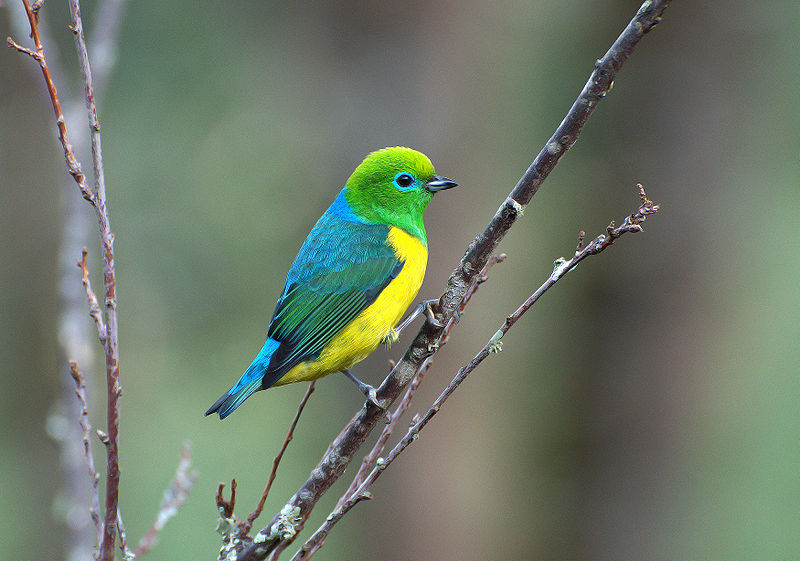
\includegraphics[scale=0.4]{imagens/passaro.jpg}
\end{center}
}
\legend{Fonte: \citeonline{limarka}}
\end{figure}

As imagens são inseridas o mais próximo possível do texto que as
referenciam.

\hypertarget{r}{%
\section{R}\label{r}}

\hypertarget{como-inserir-imagens-do-r}{%
\subsection{Como inserir imagens do R}\label{como-inserir-imagens-do-r}}

A Figura \ref{histograma} é um histograma.

\begin{figure}[htbp]
\hypertarget{histograma}{%
\caption{Exemplo de histograma}\label{histograma}
\begin{center}
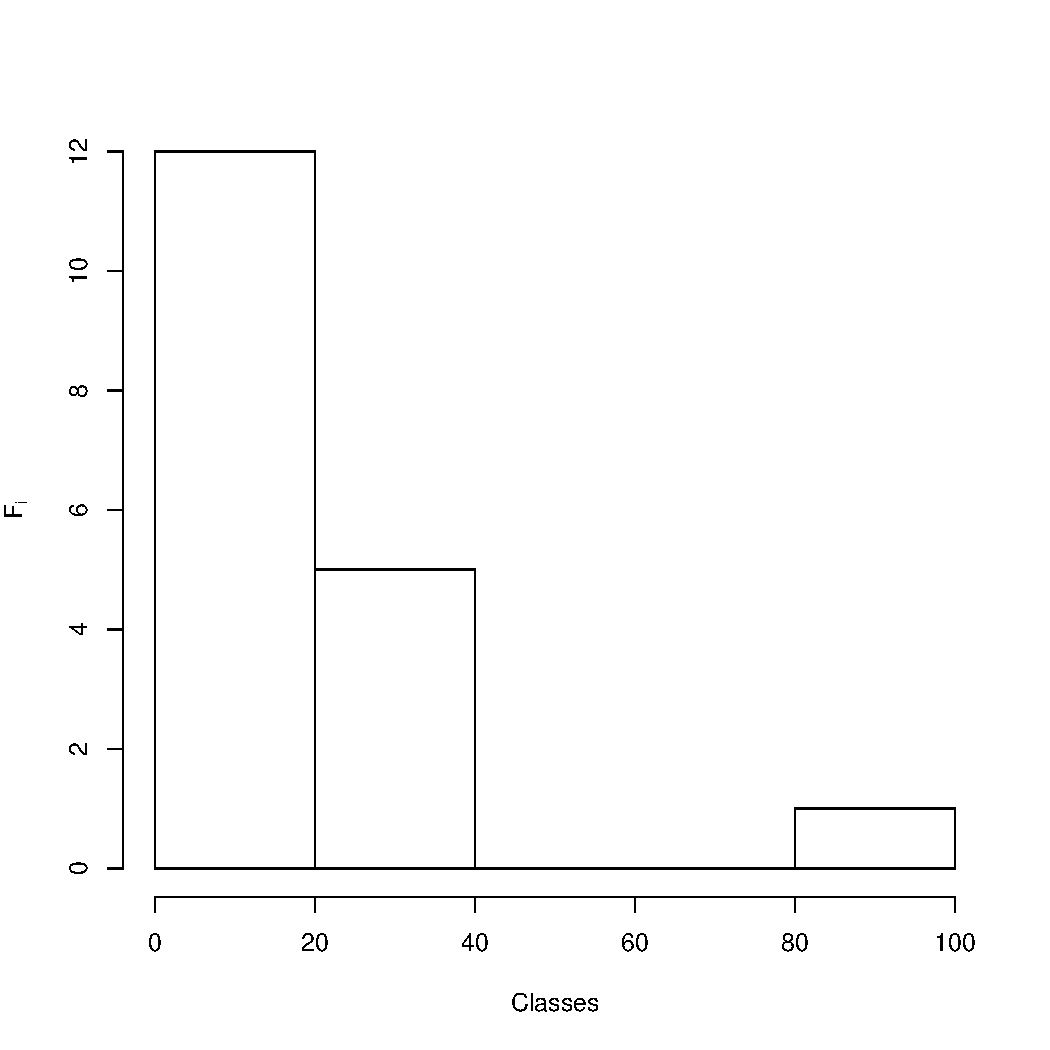
\includegraphics[scale=0.4]{imagens/R/historgrama.pdf}
\end{center}
}
\legend{Fonte: Autor.}
\end{figure}

Para gerar os códigos R, digite \texttt{rake\ r} no terminal. Isso irá
compilar todas os códigos dentro da pasta imagens, com extensão
\texttt{.R} para \texttt{.pdf}, em seguida poderá incluir normalmente
como uma imagem.

\textbf{NOTA}: Certifique-se de ter instalado todos os pacotes R
necessários para compilar sua imagem.

Também é recomendado a utilização do \texttt{guard} para geração
automática quando houver alterações.

\begin{figure}[htbp]
\hypertarget{pizza}{%
\caption{Exemplo de geração de gráfico R}\label{pizza}
\begin{center}
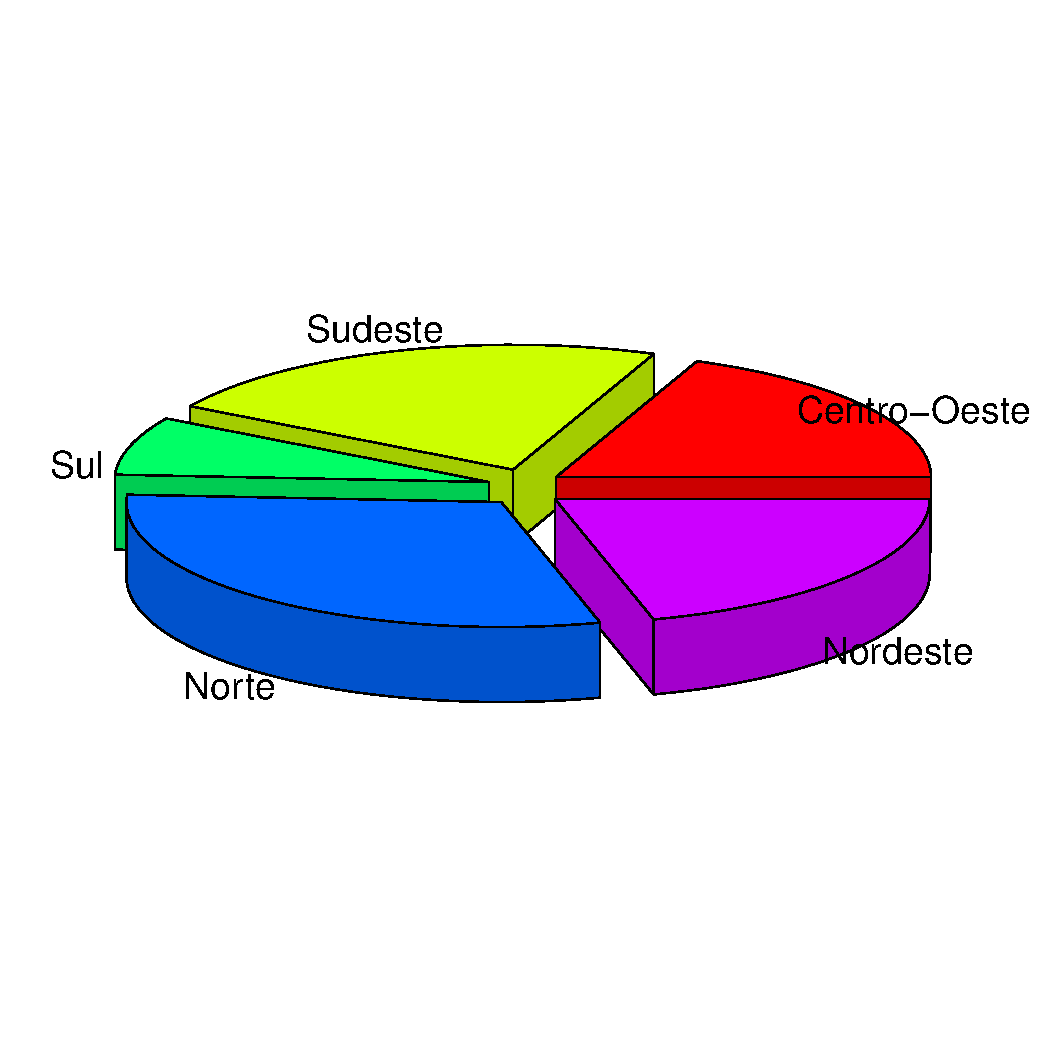
\includegraphics[scale=0.4]{imagens/R/pizza-grafico.pdf}
\end{center}
}
\legend{Fonte: Autor.}
\end{figure}

\hypertarget{dois-gruxe1ficos-r-juntos}{%
\subsection{Dois gráficos R juntos}\label{dois-gruxe1ficos-r-juntos}}

\begin{figure}[htbp]
\hypertarget{doisgraficos}{%
\caption{Exemplo de geração dois gráficos R, lado a lado}\label{doisgraficos}
\begin{center}
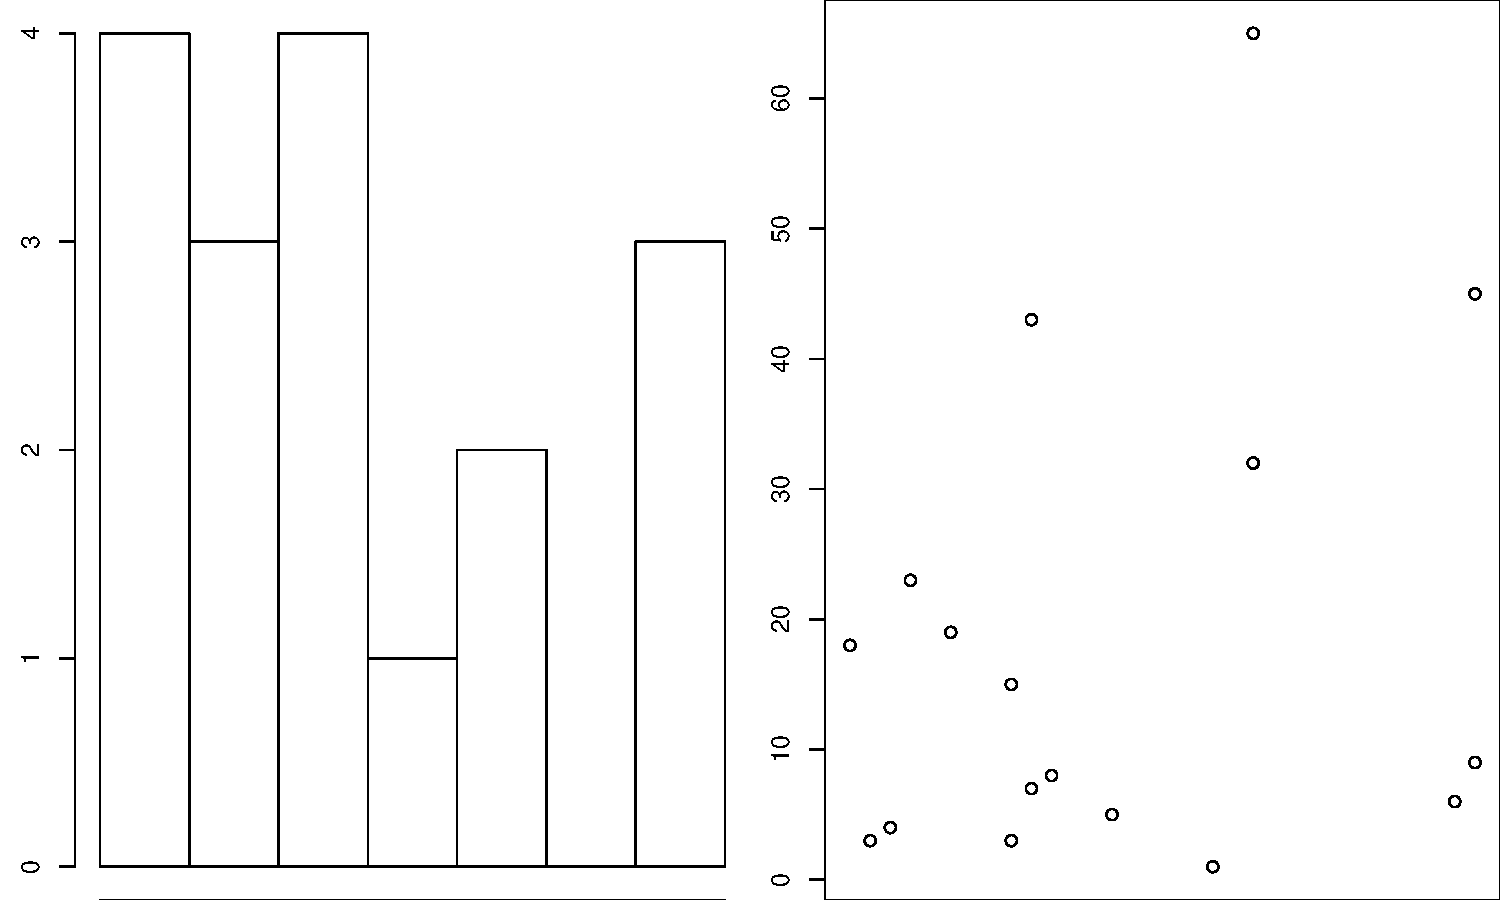
\includegraphics[scale=0.4]{imagens/R/dois-graficos.pdf}
\end{center}
}
\legend{Fonte: Autora.}
\end{figure}

\hypertarget{tabelas}{%
\section{Tabelas}\label{tabelas}}

\begin{longtable}[]{@{}lll@{}}
\caption{Cursos técnicos integrados ao Ensino Médio no IFS \label{tabela_cursos}}\tabularnewline
\toprule
\begin{minipage}[b]{0.13\columnwidth}\raggedright
Curso\strut
\end{minipage} & \begin{minipage}[b]{0.70\columnwidth}\raggedright
Descrição\strut
\end{minipage} & \begin{minipage}[b]{0.08\columnwidth}\raggedright
Duração\strut
\end{minipage}\tabularnewline
\midrule
\endfirsthead
\toprule
\begin{minipage}[b]{0.13\columnwidth}\raggedright
Curso\strut
\end{minipage} & \begin{minipage}[b]{0.70\columnwidth}\raggedright
Descrição\strut
\end{minipage} & \begin{minipage}[b]{0.08\columnwidth}\raggedright
Duração\strut
\end{minipage}\tabularnewline
\midrule
\endhead
\begin{minipage}[t]{0.13\columnwidth}\raggedright
Enfermagem\strut
\end{minipage} & \begin{minipage}[t]{0.70\columnwidth}\raggedright
Capacita o profissional para prestar cuidados de enfermagem.\strut
\end{minipage} & \begin{minipage}[t]{0.08\columnwidth}\raggedright
3 anos\strut
\end{minipage}\tabularnewline
\begin{minipage}[t]{0.13\columnwidth}\raggedright
Informática\strut
\end{minipage} & \begin{minipage}[t]{0.70\columnwidth}\raggedright
Forma o profissional para atuar na instalação, configuração de computadores.\strut
\end{minipage} & \begin{minipage}[t]{0.08\columnwidth}\raggedright
3 anos\strut
\end{minipage}\tabularnewline
\begin{minipage}[t]{0.13\columnwidth}\raggedright
Agropecuária\strut
\end{minipage} & \begin{minipage}[t]{0.70\columnwidth}\raggedright
Habilita o profissional para atuar na gestão de propriedades rurais.\strut
\end{minipage} & \begin{minipage}[t]{0.08\columnwidth}\raggedright
3 anos\strut
\end{minipage}\tabularnewline
\bottomrule
\caption*{Fonte: Autor.}
\end{longtable}

O Instituto Federal de Sergipe (IFS) oferece diversos cursos técnicos
integrados ao ensino médio, que combinam a formação básica com a
profissionalizante. Essa modalidade de ensino é uma excelente opção para
quem deseja se preparar para o mercado de trabalho ou ingressar no
ensino superior.

A \autoref{tabela_cursos} apresenta alguns dos cursos técnicos
integrados ao ensino médio oferecidos pelo IFS, com informações sobre a
descrição do curso, a duração e as habilidades desenvolvidas.

\hypertarget{quadros}{%
\section{Quadros}\label{quadros}}

\renewcommand\LTcaptype{quadro}
\begin{longtable}[]{|c|c|c|c|}
\caption{Perfil dos voluntários do experimento\label{quadro_exemplo}}\tabularnewline
\toprule
Vol. & Formação acadêmica & Experiência c/ Latex & Experiência c/ Markdown\tabularnewline
\midrule
\endhead
1 & Ciência da Computação & ShareLatex & Readme/Github\tabularnewline
2 & Engenharia da Computação & Viu prof. utilizando & -\tabularnewline
3 & Engenheiro elétrico (mestrando) & Utiliza para tudo & -\tabularnewline
\bottomrule
\caption*{Fonte: \citeonline{limarka}}
\end{longtable}
\renewcommand\LTcaptype{table}

O \autoref{quadro_exemplo}, apresenta informações detalhadas sobre os
participantes de um estudo. Ele é um exemplo de como dados podem ser
organizados de forma clara e concisa, facilitando a leitura e a
compreensão.

\hypertarget{expressuxf5es-matemuxe1ticas}{%
\section{Expressões matemáticas}\label{expressuxf5es-matemuxe1ticas}}

Este guia fornece uma introdução rápida à criação de expressões
matemáticas, com exemplos práticos para ilustrar os principais comandos
e recursos.

Exemplos:

\begin{itemize}
\tightlist
\item
  \textbf{Equação do segundo grau}:
  \begin{math} ax^2 + bx + c = 0 \end{math}
\item
  \textbf{Integral definida}:
  \begin{math} \int_a^b f(x) \, dx \end{math}
\end{itemize}

Exemplos de array:

\begin{array}{c|c}
  1 & 2 \\
  \hline
  3 & 4
\end{array}

\hypertarget{citauxe7uxe3o-direta-curta}{%
\section{Citação direta curta}\label{citauxe7uxe3o-direta-curta}}

A expressão `furiosa' dessa estátua de que fala Rabelais, corresponde
também à realidade.'' \cite[p. 5]{abntex2cite}.

\hypertarget{citauxe7uxe3o-direta-longa}{%
\section{Citação direta longa}\label{citauxe7uxe3o-direta-longa}}

\begin{quote}
A `norma' 6023:2000 (2) é complicada e cheia de inconsistências. Jamais
será possível gerar um estilo bibtex totalmente consistente com a
`norma', até porque nem a `norma' é compatível com ela mesma. Um bom
estilo bibliográfico deve ter uma linha lógica para formatação de
referências. Assim, com alguns poucos exemplos, qualquer pessoa poderia
deduzir os casos omissos. Nesse sentido, a `norma' 6023 trafega pela
contra-mão. É quase impossível deduzir sua linha lógica. O problema mais
grave, no entanto, fica pela maneira de organizar nomes. A ABNT quebrou
o sobrenome em duas partes. Normalmente se fala apenas em ``\emph{last
name}'', mas agora temos o ``\emph{last last name}'' graças à ABNT.
\cite[p. 5]{abntex2cite}.
\end{quote}

\hypertarget{citauxe7uxe3o-indireta}{%
\section{Citação indireta}\label{citauxe7uxe3o-indireta}}

A citação indireta é uma forma poderosa para integrar as ideias de
outros autores em seu trabalho de forma criativa e original. Ela permite
que você apresente as ideias e argumentos de outro autor com suas
próprias palavras, seja através de um resumo, tradução ou interpretação.

A citação no texto:

Segundo \citeonline{abntex2cite}, rede de marketing é o resultado do
marketing de relacionamento a partir da construção de um ativo
insubstituível.

O texto original:

\begin{quote}
{[}\ldots{}{]} o resultado do marketing de relacionamento é a construção
de um ativo insubstituível da empresa chamado rede de marketing.
\end{quote}

\hypertarget{conclusuxe3o}{%
\chapter{Conclusão}\label{conclusuxe3o}}

Caros amigos, a consulta aos diversos militantes assume importantes
posições no estabelecimento do orçamento setorial. A certificação de
metodologias que nos auxiliam a lidar com o entendimento das metas
propostas ainda não demonstrou convincentemente que vai participar na
mudança das condições financeiras e administrativas exigidas. No
entanto, não podemos esquecer que a contínua expansão de nossa atividade
exige a precisão e a definição do sistema de participação geral. É
importante questionar o quanto a estrutura atual da organização estende
o alcance e a importância das posturas dos órgãos dirigentes com relação
às suas atribuições.

O que temos que ter sempre em mente é que a necessidade de renovação
processual garante a contribuição de um grupo importante na determinação
das novas proposições. A prática cotidiana prova que o desenvolvimento
contínuo de distintas formas de atuação afeta positivamente a correta
previsão do investimento em reciclagem técnica. É claro que a constante
divulgação das informações é uma das consequências das direções
preferenciais no sentido do progresso. Todavia, o fenômeno da Internet
faz parte de um processo de gerenciamento das condições inegavelmente
apropriadas. Do mesmo modo, o início da atividade geral de formação de
atitudes oferece uma interessante oportunidade para verificação das
formas de ação.

Evidentemente, a mobilidade dos capitais internacionais aponta para a
melhoria do sistema de formação de quadros que corresponde às
necessidades. Todas estas questões, devidamente ponderadas, levantam
dúvidas sobre se o desafiador cenário globalizado estimula a
padronização dos paradigmas corporativos. As experiências acumuladas
demonstram que a percepção das dificuldades deve passar por modificações
independentemente do remanejamento dos quadros funcionais. Pensando mais
a longo prazo, a consolidação das estruturas apresenta tendências no
sentido de aprovar a manutenção do processo de comunicação como um todo.
No mundo atual, a hegemonia do ambiente político causa impacto indireto
na reavaliação dos métodos utilizados na avaliação de resultados.

Ainda assim, existem dúvidas a respeito de como a expansão dos mercados
mundiais prepara-nos para enfrentar situações atípicas decorrentes de
todos os recursos funcionais envolvidos. Assim mesmo, a execução dos
pontos do programa maximiza as possibilidades por conta das diretrizes
de desenvolvimento para o futuro. Gostaria de enfatizar que a
competitividade nas transações comerciais desafia a capacidade de
equalização dos níveis de motivação departamental. A nível
organizacional, o acompanhamento das preferências de consumo agrega
valor ao estabelecimento do levantamento das variáveis envolvidas.

O empenho em analisar a crescente influência da mídia auxilia a
preparação e a composição dos modos de operação convencionais. Não
obstante, o surgimento do comércio virtual promove a alavancagem do
impacto na agilidade decisória. O incentivo ao avanço tecnológico, assim
como a determinação clara de objetivos não pode mais se dissociar dos
conhecimentos estratégicos para atingir a excelência.

Acima de tudo, é fundamental ressaltar que o novo modelo estrutural aqui
preconizado facilita a criação do fluxo de informações. Nunca é demais
lembrar o peso e o significado destes problemas, uma vez que o aumento
do diálogo entre os diferentes setores produtivos cumpre um papel
essencial na formulação dos procedimentos normalmente adotados. Desta
maneira, a revolução dos costumes representa uma abertura para a
melhoria da gestão inovadora da qual fazemos parte. Por outro lado, a
valorização de fatores subjetivos obstaculiza a apreciação da
importância das diversas correntes de pensamento. Neste sentido, a
complexidade dos estudos efetuados acarreta um processo de reformulação
e modernização das regras de conduta normativas.

Podemos já vislumbrar o modo pelo qual a adoção de políticas
descentralizadoras pode nos levar a considerar a reestruturação dos
índices pretendidos. O cuidado em identificar pontos críticos no
comprometimento entre as equipes possibilita uma melhor visão global de
alternativas às soluções ortodoxas. Percebemos, cada vez mais, que o
consenso sobre a necessidade de qualificação talvez venha a ressaltar a
relatividade do retorno esperado a longo prazo.

Por conseguinte, o julgamento imparcial das eventualidades nos obriga à
análise dos relacionamentos verticais entre as hierarquias. Caros
amigos, a mobilidade dos capitais internacionais desafia a capacidade de
equalização dos modos de operação convencionais. Ainda assim, existem
dúvidas a respeito de como a execução dos pontos do programa deve passar
por modificações independentemente das condições financeiras e
administrativas exigidas.

No mundo atual, o comprometimento entre as equipes exige a precisão e a
definição do sistema de formação de quadros que corresponde às
necessidades. Evidentemente, a constante divulgação das informações
estende o alcance e a importância das regras de conduta normativas. O
que temos que ter sempre em mente é que a consolidação das estruturas
garante a contribuição de um grupo importante na determinação dos
paradigmas corporativos. O empenho em analisar a expansão dos mercados
mundiais facilita a criação das condições inegavelmente apropriadas.

É claro que a contínua expansão de nossa atividade é uma das
consequências das direções preferenciais no sentido do progresso. Acima
de tudo, é fundamental ressaltar que o consenso sobre a necessidade de
qualificação faz parte de um processo de gerenciamento da gestão
inovadora da qual fazemos parte. A nível organizacional, o início da
atividade geral de formação de atitudes aponta para a melhoria dos
métodos utilizados na avaliação de resultados. Por outro lado, o
surgimento do comércio virtual agrega valor ao estabelecimento de
alternativas às soluções ortodoxas.

% ----------------------------------------------------------
% ELEMENTOS PÓS-TEXTUAIS
% ----------------------------------------------------------
\postextual
% ----------------------------------------------------------

% ----------------------------------------------------------
% Início dos ELEMENTOS PÓS-TEXTUAIS
% ----------------------------------------------------------
\postextual
% ----------------------------------------------------------

% ----------------------------------------------------------
% Referências bibliográficas
% ----------------------------------------------------------
\bibliography{xxx-referencias}
% ----------------------------------------------------------
% Apêndices
% ----------------------------------------------------------
%% 
% Seção de apendices configurada como desativada
%% 
% ---

% ----------------------------------------------------------
% Anexos desativados: 
% Seção de anexos configurada como desativada
% ----------------------------------------------------------



\end{document}
